%% fig_speciallocus.tex   (generated by make_round37.py; do not edit by hand)
%% The special locus (prop:speciallocus) and an escaping sequence of CM points (thm:escape).
\documentclass[tikz,border=8pt]{standalone}
\usepackage{amsmath,amssymb}
\usetikzlibrary{arrows.meta,calc,decorations.pathreplacing}
%% palette.tex -- shared colour definitions for the figures
\definecolor{PInk}{RGB}{26,32,44}
\definecolor{PBlue}{RGB}{37,82,139}
\definecolor{PTeal}{RGB}{23,127,125}
\definecolor{POchre}{RGB}{193,138,44}
\definecolor{PClay}{RGB}{178,74,58}
\definecolor{PSlate}{RGB}{108,122,137}
\definecolor{PViolet}{RGB}{110,86,150}
\definecolor{WBlue}{RGB}{223,234,246}
\definecolor{WTeal}{RGB}{220,238,236}
\definecolor{WOchre}{RGB}{250,240,218}
\definecolor{WClay}{RGB}{247,229,224}
\definecolor{WSlate}{RGB}{238,241,244}
\definecolor{PMag}{RGB}{158,58,110}
\definecolor{PGrass}{RGB}{62,124,66}
\definecolor{PAmber}{RGB}{214,112,38}
\definecolor{PIndigo}{RGB}{58,64,140}
\definecolor{PRule}{RGB}{176,186,197}

%% shared macros so the standalone figures match the paper
\providecommand{\QQ}{\mathbb{Q}}
\providecommand{\ZZ}{\mathbb{Z}}
\providecommand{\RR}{\mathbb{R}}
\providecommand{\CC}{\mathbb{C}}
\providecommand{\PP}{\mathbb{P}}
\providecommand{\Kx}{K^{\times}}
\providecommand{\HW}{W}
\providecommand{\Nm}{\mathrm{N}}
\providecommand{\Hdg}{\mathrm{Hdg}}
\providecommand{\NS}{\mathrm{NS}}
\providecommand{\cA}{\mathcal{A}}
\providecommand{\cD}{\mathcal{D}}
\providecommand{\cF}{\mathcal{F}}
\providecommand{\cP}{\mathcal{P}}
\providecommand{\cO}{\mathcal{O}}
\providecommand{\cQ}{\mathcal{Q}}
\providecommand{\bbar}[1]{\overline{#1}}
\providecommand{\ch}{\operatorname{ch}}
\providecommand{\End}{\mathrm{End}}
\providecommand{\Ext}{\operatorname{Ext}}
\providecommand{\Supp}{\operatorname{Supp}}

\begin{document}
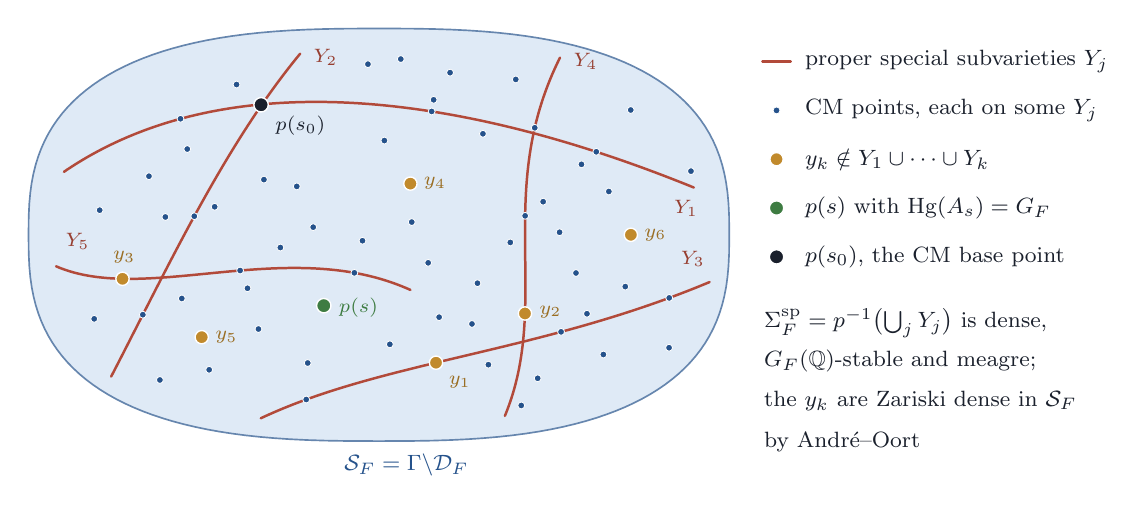
\begin{tikzpicture}[x=1cm,y=1cm,line join=round,line cap=round,
  font=\small,text=PInk,lbl/.style={inner sep=1pt}]
  \path[fill=WBlue,draw=PBlue!70,line width=0.60pt] (9.0000,2.7500) -- (8.9975,2.9881) -- (8.9898,3.1477) -- (8.9771,3.2865) -- (8.9594,3.4130) -- (8.9365,3.5308) -- (8.9086,3.6418) -- (8.8756,3.7472) -- (8.8376,3.8478) -- (8.7946,3.9439) -- (8.7465,4.0362) -- (8.6935,4.1247) -- (8.6354,4.2097) -- (8.5724,4.2914) -- (8.5044,4.3699) -- (8.4314,4.4452) -- (8.3535,4.5175) -- (8.2706,4.5867) -- (8.1828,4.6530) -- (8.0901,4.7164) -- (7.9924,4.7768) -- (7.8898,4.8343) -- (7.7822,4.8889) -- (7.6696,4.9406) -- (7.5520,4.9893) -- (7.4292,5.0352) -- (7.3013,5.0782) -- (7.1680,5.1182) -- (7.0293,5.1553) -- (6.8848,5.1895) -- (6.7345,5.2208) -- (6.5779,5.2491) -- (6.4145,5.2744) -- (6.2438,5.2968) -- (6.0648,5.3162) -- (5.8762,5.3326) -- (5.6761,5.3461) -- (5.4612,5.3565) -- (5.2254,5.3640) -- (4.9544,5.3685) -- (4.5500,5.3700) -- (4.1456,5.3685) -- (3.8746,5.3640) -- (3.6388,5.3565) -- (3.4239,5.3461) -- (3.2238,5.3326) -- (3.0352,5.3162) -- (2.8562,5.2968) -- (2.6855,5.2744) -- (2.5221,5.2491) -- (2.3655,5.2208) -- (2.2152,5.1895) -- (2.0707,5.1553) -- (1.9320,5.1182) -- (1.7987,5.0782) -- (1.6708,5.0352) -- (1.5480,4.9893) -- (1.4304,4.9406) -- (1.3178,4.8889) -- (1.2102,4.8343) -- (1.1076,4.7768) -- (1.0099,4.7164) -- (0.9172,4.6530) -- (0.8294,4.5867) -- (0.7465,4.5175) -- (0.6686,4.4452) -- (0.5956,4.3699) -- (0.5276,4.2914) -- (0.4646,4.2097) -- (0.4065,4.1247) -- (0.3535,4.0362) -- (0.3054,3.9439) -- (0.2624,3.8478) -- (0.2244,3.7472) -- (0.1914,3.6418) -- (0.1635,3.5308) -- (0.1406,3.4130) -- (0.1229,3.2865) -- (0.1102,3.1477) -- (0.1025,2.9881) -- (0.1000,2.7500) -- (0.1025,2.5119) -- (0.1102,2.3523) -- (0.1229,2.2135) -- (0.1406,2.0870) -- (0.1635,1.9692) -- (0.1914,1.8582) -- (0.2244,1.7528) -- (0.2624,1.6522) -- (0.3054,1.5561) -- (0.3535,1.4638) -- (0.4065,1.3753) -- (0.4646,1.2903) -- (0.5276,1.2086) -- (0.5956,1.1301) -- (0.6686,1.0548) -- (0.7465,0.9825) -- (0.8294,0.9133) -- (0.9172,0.8470) -- (1.0099,0.7836) -- (1.1076,0.7232) -- (1.2102,0.6657) -- (1.3178,0.6111) -- (1.4304,0.5594) -- (1.5480,0.5107) -- (1.6708,0.4648) -- (1.7987,0.4218) -- (1.9320,0.3818) -- (2.0707,0.3447) -- (2.2152,0.3105) -- (2.3655,0.2792) -- (2.5221,0.2509) -- (2.6855,0.2256) -- (2.8562,0.2032) -- (3.0352,0.1838) -- (3.2238,0.1674) -- (3.4239,0.1539) -- (3.6388,0.1435) -- (3.8746,0.1360) -- (4.1456,0.1315) -- (4.5500,0.1300) -- (4.9544,0.1315) -- (5.2254,0.1360) -- (5.4612,0.1435) -- (5.6761,0.1539) -- (5.8762,0.1674) -- (6.0648,0.1838) -- (6.2438,0.2032) -- (6.4145,0.2256) -- (6.5779,0.2509) -- (6.7345,0.2792) -- (6.8848,0.3105) -- (7.0293,0.3447) -- (7.1680,0.3818) -- (7.3013,0.4218) -- (7.4292,0.4648) -- (7.5520,0.5107) -- (7.6696,0.5594) -- (7.7822,0.6111) -- (7.8898,0.6657) -- (7.9924,0.7232) -- (8.0901,0.7836) -- (8.1828,0.8470) -- (8.2706,0.9133) -- (8.3535,0.9825) -- (8.4314,1.0548) -- (8.5044,1.1301) -- (8.5724,1.2086) -- (8.6354,1.2903) -- (8.6935,1.3753) -- (8.7465,1.4638) -- (8.7946,1.5561) -- (8.8376,1.6522) -- (8.8756,1.7528) -- (8.9086,1.8582) -- (8.9365,1.9692) -- (8.9594,2.0870) -- (8.9771,2.2135) -- (8.9898,2.3523) -- (8.9975,2.5119) -- cycle;
  \draw[PClay,line width=0.9pt] (0.5500,3.5500) .. controls (2.6000,4.9500) and (5.6000,4.5500) .. (8.5500,3.3500);
  \draw[PClay,line width=0.9pt] (1.1500,0.9500) .. controls (1.9000,2.4000) and (2.6000,3.9000) .. (3.5500,5.0500);
  \draw[PClay,line width=0.9pt] (3.0500,0.4200) .. controls (4.6000,1.1500) and (6.6000,1.2500) .. (8.7500,2.1500);
  \draw[PClay,line width=0.9pt] (6.1500,0.4500) .. controls (6.7500,1.9000) and (6.0000,3.3000) .. (6.8500,5.0000);
  \draw[PClay,line width=0.9pt] (0.4500,2.3500) .. controls (1.6000,1.8500) and (3.4000,2.7500) .. (4.9500,2.0500);
  \path[fill=PBlue,draw=white,line width=0.30pt] (2.8812,2.0707) circle (1.25pt);
  \path[fill=PBlue,draw=white,line width=0.30pt] (1.7687,0.9063) circle (1.25pt);
  \path[fill=PBlue,draw=white,line width=0.30pt] (6.2188,2.6530) circle (1.25pt);
  \path[fill=PBlue,draw=white,line width=0.30pt] (4.8281,4.9819) circle (1.25pt);
  \path[fill=PBlue,draw=white,line width=0.30pt] (7.0531,2.2648) circle (1.25pt);
  \path[fill=PBlue,draw=white,line width=0.30pt] (5.9406,1.1004) circle (1.25pt);
  \path[fill=PBlue,draw=white,line width=0.30pt] (3.7156,2.8470) circle (1.25pt);
  \path[fill=PBlue,draw=white,line width=0.30pt] (0.9344,1.6826) circle (1.25pt);
  \path[fill=PBlue,draw=white,line width=0.30pt] (2.0469,1.9414) circle (1.25pt);
  \path[fill=PBlue,draw=white,line width=0.30pt] (4.6891,1.3591) circle (1.25pt);
  \path[fill=PBlue,draw=white,line width=0.30pt] (2.4641,3.1058) circle (1.25pt);
  \path[fill=PBlue,draw=white,line width=0.30pt] (5.8016,2.1354) circle (1.25pt);
  \path[fill=PBlue,draw=white,line width=0.30pt] (5.2453,4.4643) circle (1.25pt);
  \path[fill=PBlue,draw=white,line width=0.30pt] (3.0203,1.5532) circle (1.25pt);
  \path[fill=PBlue,draw=white,line width=0.30pt] (7.4703,3.2999) circle (1.25pt);
  \path[fill=PBlue,draw=white,line width=0.30pt] (6.3578,0.5828) circle (1.25pt);
  \path[fill=PBlue,draw=white,line width=0.30pt] (4.9672,2.9117) circle (1.25pt);
  \path[fill=PBlue,draw=white,line width=0.30pt] (2.7422,4.6584) circle (1.25pt);
  \path[fill=PBlue,draw=white,line width=0.30pt] (7.1922,1.7473) circle (1.25pt);
  \path[fill=PBlue,draw=white,line width=0.30pt] (1.6297,3.4940) circle (1.25pt);
  \path[fill=PBlue,draw=white,line width=0.30pt] (3.2984,2.5883) circle (1.25pt);
  \path[fill=PBlue,draw=white,line width=0.30pt] (7.7484,4.3349) circle (1.25pt);
  \path[fill=PBlue,draw=white,line width=0.30pt] (6.6359,3.1705) circle (1.25pt);
  \path[fill=PBlue,draw=white,line width=0.30pt] (4.4109,4.9172) circle (1.25pt);
  \path[fill=PBlue,draw=white,line width=0.30pt] (4.6195,3.9468) circle (1.25pt);
  \path[fill=PBlue,draw=white,line width=0.30pt] (2.3945,1.0357) circle (1.25pt);
  \path[fill=PBlue,draw=white,line width=0.30pt] (6.8445,2.7823) circle (1.25pt);
  \path[fill=PBlue,draw=white,line width=0.30pt] (5.7320,1.6179) circle (1.25pt);
  \path[fill=PBlue,draw=white,line width=0.30pt] (3.5070,3.3646) circle (1.25pt);
  \path[fill=PBlue,draw=white,line width=0.30pt] (5.1758,2.3942) circle (1.25pt);
  \path[fill=PBlue,draw=white,line width=0.30pt] (7.4008,1.2298) circle (1.25pt);
  \path[fill=PBlue,draw=white,line width=0.30pt] (1.8383,2.9764) circle (1.25pt);
  \path[fill=PBlue,draw=white,line width=0.30pt] (6.2883,4.7231) circle (1.25pt);
  \path[fill=PBlue,draw=white,line width=0.30pt] (8.5133,3.5586) circle (1.25pt);
  \path[fill=PBlue,draw=white,line width=0.30pt] (7.1227,3.6449) circle (1.25pt);
  \path[fill=PBlue,draw=white,line width=0.30pt] (8.2352,1.3160) circle (1.25pt);
  \path[fill=PBlue,draw=white,line width=0.30pt] (1.0039,3.0627) circle (1.25pt);
  \path[fill=PBlue,draw=white,line width=0.30pt] (5.4539,4.8093) circle (1.25pt);
  \path[fill=PBlue,draw=white,line width=0.30pt] (7.6789,2.0923) circle (1.25pt);
  \path[fill=PBlue,draw=white,line width=0.30pt] (2.1164,3.8390) circle (1.25pt);
  \path[fill=PBlue,draw=white,line width=0.30pt] (6.5664,0.9279) circle (1.25pt);
  \path[fill=PBlue,draw=white,line width=0.30pt] (4.3414,2.6745) circle (1.25pt);
  \path[fill=PBlue,draw=white,line width=0.30pt] (5.8711,4.0330) circle (1.25pt);
  \path[fill=PBlue,draw=white,line width=0.30pt] (3.6461,1.1219) circle (1.25pt);
  \path[fill=PBlue,draw=white,line width=0.30pt] (5.3148,1.7042) circle (1.25pt);
  \path[fill=PBlue,draw=white,line width=0.30pt] (3.0898,3.4508) circle (1.25pt);
  \path[fill=PBlue,draw=white,line width=0.30pt] (2.0303,4.2233) circle (1.25pt);
  \path[fill=PBlue,draw=white,line width=0.30pt] (5.2202,4.3166) circle (1.25pt);
  \path[fill=PBlue,draw=white,line width=0.30pt] (7.3108,3.8042) circle (1.25pt);
  \path[fill=PBlue,draw=white,line width=0.30pt] (1.5519,1.7355) circle (1.25pt);
  \path[fill=PBlue,draw=white,line width=0.30pt] (2.2055,2.9861) circle (1.25pt);
  \path[fill=PBlue,draw=white,line width=0.30pt] (3.6269,0.6581) circle (1.25pt);
  \path[fill=PBlue,draw=white,line width=0.30pt] (6.8636,1.5174) circle (1.25pt);
  \path[fill=PBlue,draw=white,line width=0.30pt] (8.2370,1.9486) circle (1.25pt);
  \path[fill=PBlue,draw=white,line width=0.30pt] (6.4072,2.9908) circle (1.25pt);
  \path[fill=PBlue,draw=white,line width=0.30pt] (6.5293,4.1091) circle (1.25pt);
  \path[fill=PBlue,draw=white,line width=0.30pt] (2.7876,2.2964) circle (1.25pt);
  \path[fill=PBlue,draw=white,line width=0.30pt] (4.2387,2.2671) circle (1.25pt);
  \path[fill=PInk,draw=white,line width=0.50pt] (3.0536,4.4013) circle (2.60pt);
  \path[fill=POchre,draw=white,line width=0.50pt] (5.2753,1.1259) circle (2.40pt);
  \path[fill=POchre,draw=white,line width=0.50pt] (6.4051,1.7509) circle (2.40pt);
  \path[fill=POchre,draw=white,line width=0.50pt] (1.2938,2.1913) circle (2.40pt);
  \path[fill=POchre,draw=white,line width=0.50pt] (4.9500,3.4000) circle (2.40pt);
  \path[fill=POchre,draw=white,line width=0.50pt] (2.3000,1.4500) circle (2.40pt);
  \path[fill=POchre,draw=white,line width=0.50pt] (7.7500,2.7500) circle (2.40pt);
  \path[fill=PGrass,draw=white,line width=0.50pt] (3.8500,1.8500) circle (2.60pt);
  \draw[PClay,line width=0.9pt] (9.4200,4.9500) -- (9.7800,4.9500);
  \path[fill=PBlue,draw=white,line width=0.30pt] (9.6000,4.3300) circle (1.25pt);
  \path[fill=POchre,draw=white,line width=0.50pt] (9.6000,3.7100) circle (2.40pt);
  \path[fill=PGrass,draw=white,line width=0.50pt] (9.6000,3.0900) circle (2.60pt);
  \path[fill=PInk,draw=white,line width=0.50pt] (9.6000,2.4700) circle (2.60pt);
  \node[lbl,anchor=north,text=PBlue,font=\footnotesize] at (4.9000,0.0100) {$\mathcal{S}_{F}=\Gamma\backslash\cD_{F}$};
  \node[lbl,anchor=north,text=PClay!85!black,font=\scriptsize] at (8.4500,3.2300) {$Y_{1}$};
  \node[lbl,anchor=west,text=PClay!85!black,font=\scriptsize] at (3.6800,5.0000) {$Y_{2}$};
  \node[lbl,anchor=east,text=PClay!85!black,font=\scriptsize] at (8.7300,2.4438) {$Y_{3}$};
  \node[lbl,anchor=west,text=PClay!85!black,font=\scriptsize] at (6.9800,4.9500) {$Y_{4}$};
  \node[lbl,anchor=west,text=PClay!85!black,font=\scriptsize] at (0.5300,2.6638) {$Y_{5}$};
  \node[lbl,anchor=west,text=PInk,font=\scriptsize] at (3.1936,4.1361) {$p(s_{0})$};
  \node[lbl,anchor=west,text=POchre!80!black,font=\scriptsize] at (5.3953,0.8769) {$y_{1}$};
  \node[lbl,anchor=west,text=POchre!80!black,font=\scriptsize] at (6.5451,1.7709) {$y_{2}$};
  \node[lbl,anchor=south,text=POchre!80!black,font=\scriptsize] at (1.3138,2.3413) {$y_{3}$};
  \node[lbl,anchor=west,text=POchre!80!black,font=\scriptsize] at (5.0800,3.4000) {$y_{4}$};
  \node[lbl,anchor=west,text=POchre!80!black,font=\scriptsize] at (2.4300,1.4500) {$y_{5}$};
  \node[lbl,anchor=west,text=POchre!80!black,font=\scriptsize] at (7.8800,2.7500) {$y_{6}$};
  \node[lbl,anchor=west,text=PGrass,font=\scriptsize] at (4.0000,1.8300) {$p(s)$};
  \node[lbl,anchor=west,text=PInk,font=\footnotesize] at (9.9200,4.9500) {proper special subvarieties $Y_{j}$};
  \node[lbl,anchor=west,text=PInk,font=\footnotesize] at (9.9200,4.3300) {CM points, each on some $Y_{j}$};
  \node[lbl,anchor=west,text=PInk,font=\footnotesize] at (9.9200,3.7100) {$y_{k}\notin Y_{1}\cup\dots\cup Y_{k}$};
  \node[lbl,anchor=west,text=PInk,font=\footnotesize] at (9.9200,3.0900) {$p(s)$ with $\mathrm{Hg}(A_{s})=G_{F}$};
  \node[lbl,anchor=west,text=PInk,font=\footnotesize] at (9.9200,2.4700) {$p(s_{0})$, the CM base point};
  \node[lbl,anchor=west,text=PInk,font=\footnotesize] at (9.4000,1.6239) {$\Sigma^{\mathrm{sp}}_{F}=p^{-1}\bigl(\bigcup_{j}Y_{j}\bigr)$ is dense,};
  \node[lbl,anchor=west,text=PInk,font=\footnotesize] at (9.4000,1.1472) {$G_{F}(\QQ)$-stable and meagre;};
  \node[lbl,anchor=west,text=PInk,font=\footnotesize] at (9.4000,0.6429) {the $y_{k}$ are Zariski dense in $\mathcal{S}_{F}$};
  \node[lbl,anchor=west,text=PInk,font=\footnotesize] at (9.4000,0.1229) {by Andr\'e--Oort};
\end{tikzpicture}
\end{document}
